\pdfoutput=1
\documentclass{llncs}
\usepackage[T1]{fontenc}
\usepackage{newtxtext}
\usepackage[varvw]{newtxmath}
\usepackage{graphicx}
\usepackage{booktabs}
\usepackage{placeins}
\usepackage[hidelinks]{hyperref}
\pdfmapfile{+newtx.map}
\pdfmapfile{+qtm.map}
\pdfmapfile{+txfonts.map}
\pdfmapfile{+cm.map}
\hypersetup{pdftitle={Efficient Solar-Access Intervention Screening for Early Urban Renewal: An Auditable Decision-Support Workflow},pdfauthor={},pdfsubject={Anonymous regular-paper manuscript for author review},pdfkeywords={solar access, decision support, exhaustive screening, geometry validation},pdfcreator={LaTeX}}
\pdfinfoomitdate=1
\pdftrailerid{}
\newcommand{\aidraft}{\footnote{Substantial AI-assisted text preparation in this section~\cite{openai2026}; see the AI-Assistance Disclosure.}}
\providecommand{\Description}[1]{}
\newcommand{\ind}{\mathbf{1}}
\begin{document}
\title{Efficient Solar-Access Intervention Screening for Early Urban Renewal: An Auditable Decision-Support Workflow}
\author{}
\institute{}
\maketitle
\begin{abstract}
Architects considering solar-access improvements in an existing urban block need a manageable set of alternatives before investing in detailed design and simulation. This paper presents a bounded, auditable screening workflow: 630 rule-based two-building height-reduction candidates are ranked by declared preferences and an area--volume Pareto analysis; a curated set of 23 receives archived Honeybee/Radiance review; geometric translation and professional judgment remain separate gates. The case contains 45 building groups, of which 36 are eligible under research constraints. We report the actual top-ten shortlist with its performance, nominal volume costs and review status, rather than treating the candidates as completed architectural designs. A separately frozen 20-candidate same-site coverage cohort has low-sun-area mean absolute error of 0.45~m$^2$, resulting from one 9~m$^2$ grid-cell discrepancy. Historical matched tests support fast exhaustive screening: median full-universe runtime falls from 11,608.183 to 24.037~s through blocker reuse, including precomputation, for two specific single-thread implementations. Historical translation replays also expose outside-footprint walls; four contained corrections remove the observed adverse sunlight events. Current cloud work reanalyses archived aggregates and does not perform new site simulations. The contribution is an evidence-linked choice set for further architectural assessment, conditional on approximate canonical geometry, a fixed sampling protocol and explicit preferences. AI assistance in preparing this abstract is disclosed~\cite{openai2026}.
\keywords{Decision support \and Solar access \and Urban renewal \and Candidate screening \and Multi-criteria evaluation}
\end{abstract}

\section{Introduction}
An architect investigating an existing block rarely begins with a single intervention whose consequences are already known.\aidraft{} Several building groups may be eligible for study, and a modest rule such as reducing the height of two groups immediately creates hundreds of combinations. Detailed modeling and simulation of every alternative can consume effort before the useful trade-offs are clear. The early decision is therefore which candidates deserve closer examination, with what evidence, and under which unresolved constraints. A useful computational output is a traceable shortlist that preserves the architect's ability to question the assumptions and choose a next step.

Solar access is one part of that decision. Urban environmental analysis distinguishes irradiation, illuminance and duration of direct exposure~\cite{compagnon2004urban,czachura2022metrics}. We use sampled outdoor direct-sun hours and a research threshold to describe low-sun grid area. These quantities do not measure indoor daylight, annual energy performance or statutory compliance. Nor do they establish a right to alter the buildings represented by a model. Making these boundaries visible is part of the decision-support task rather than an incidental caveat.

This paper asks: under a fixed canonical block model and explicit low-intervention height rules, can the complete set of 630 building-pair candidates be evaluated efficiently and reduced to an auditable set for further architectural judgment? The workflow follows a deliberate sequence: define the rule universe; evaluate and rank all candidates; expose a top-ten list and complementary nondominated alternatives; review a curated set of 23 through an archived Honeybee/Radiance route; and separately assess translated geometry before any professional decision. A separately frozen 20-candidate same-site coverage cohort provides additional, limited agreement evidence. Neither cohort establishes general accuracy across cities.

The case contains 45 building groups and a research-defined eligible subset of 36. Each candidate changes exactly two heights according to one fixed rule and leaves footprints unchanged. Four metrics describe benefits and nominal intervention cost, while fixed weights express one preference scenario. These are 630 rule-based volumetric alternatives, not 630 complete designs. Likewise, the top ten are candidates for further assessment rather than ten construction-ready solutions. Ownership, use, structural safety, heritage constraints and implementation remain matters for the architect and other responsible professionals.

Three contributions serve that decision sequence. First, a fully enumerated and reproducible shortlist connects candidate identities to metrics, score, Pareto membership and review status. Second, the evidence distinguishes screening agreement, computational equivalence and design-translation validity, so that a high rank does not silently become a claim of professional approval. Third, historical matched runtime and controlled translation experiments show how reuse and containment checks support a usable, auditable screening process. The algorithm is application-specific exhaustive screening, not a trained AI system or a new general optimization method. No architect user study or realized improvement to a built street is claimed.

\section{Related Work and Positioning}
Urban solar-performance assessment has long considered the interaction between built form and the availability of sunlight and daylight.\aidraft{} Compagnon~\cite{compagnon2004urban} evaluates solar and daylight availability in urban fabric through surface-based performance analysis. The taxonomy of Czachura et al.~\cite{czachura2022metrics} helps distinguish the metrics used in urban planning. This distinction matters here: a threshold on sampled direct-sun hours cannot be substituted for irradiation, daylight autonomy or a jurisdiction-specific compliance test.

Simulation-based design-support methods already connect changes in building form to environmental objectives. Konis et al.~\cite{konis2016passive} present an optimization framework for early-stage passive-design support. De Luca et al.~\cite{deluca2021reverse} develop a reverse solar-envelope form-finding method that can accommodate regulatory frameworks. Our study has a narrower search space: it exhaustively ranks a fixed set of two-building height-reduction rules, then treats stepback generation as a separate, fallible translation. We do not benchmark against those systems or infer that exhaustive enumeration outperforms their broader form-finding methods.

The software ecosystem also supplies distinct computational roles. Ladybug supports parametric environmental analysis~\cite{roudsari2013ladybug}; Radiance provides a lighting simulation and rendering system based on ray tracing~\cite{ward1994radiance}; and pvlib supplies solar-energy modeling implementations including solar-position calculation~\cite{holmgren2018pvlib}. These references establish the context of the tools, not the validity of our particular inputs or recipe. In particular, the effective solar vectors recovered from the archived Honeybee/Ladybug route are not numerically identical to the saved pvlib vectors. Cross-route agreement therefore concerns the actual archived configurations, whereas the efficiency comparison isolates two implementations using exactly the same geometric primitive and vectors.

\section{Case, Decision Universe and Solar Setup}
\subsection{Bounded Candidate Universe}
Let $\mathcal{B}$ denote the 45 building groups, each represented by a footprint $F_i$ and height $h_i$.\aidraft{} The eligible subset $E\subset\mathcal{B}$ contains 36 groups selected using source flags for movable and protected buildings, strict Boolean parsing and $h_i>3$~m. A feasible rule decision satisfies
\begin{equation}
 z_i\in\{0,1\}\ (i\in E),\qquad \sum_{i\in E}z_i=2,
 \label{eq:select}
\end{equation}
with $z_i=0$ outside $E$. For a selected building, the rule height is
\begin{equation}
 h_i^r=\max\{3,\ h_i-\min(3,0.25h_i)\},\qquad
 h_i(z)=(1-z_i)h_i+z_i h_i^r, \label{eq:height}
\end{equation}
where heights are in metres. Thus $\binom{36}{2}=630$ unordered pairs constitute the complete declared universe. Exhaustive evaluation establishes an optimum only for a specified score within this finite universe. It says nothing about other numbers of altered buildings, alternative height rules, footprint changes, structural feasibility or legal rights.

The canonical footprints are unions of bounding boxes associated with DXF components. Some building identifiers share components and some footprints overlap. The archived OBJ representation also disagrees with the canonical model for important candidates. We retain the frozen canonical input for reproducibility, but do not describe it as a surveyed or as-built boundary model. This distinction affects both visibility and volume interpretation.

\subsection{Receiving Grid, Time Samples and Visibility}
The protocol fixes 2,031 receiving points on a 3~m horizontal grid at height 0.1~m. The geographic parameters are latitude $24.55^\circ$N and longitude $118.03^\circ$E, with UTC+8 local time and an assumed north angle of zero. The declared analysis date for the pvlib sequence is 21 December 2026, a near-solstice winter design-day scenario rather than observed future weather or a demonstrated worst case across dates. Sixteen half-hour samples are centred at 08:15, 08:45, $\ldots$, 15:45. Each carries weight $\Delta t=0.5$~h, so the total integration weight is 8~h, despite the 7.5~h span between the first and last sample centres. These are discrete samples, not continuous-time exposure measurements.

For receiver $j$ and sample $t$, let $d_t=\ind\{\alpha_t>0\}$ indicate an above-horizon solar altitude and let $b_{jt}(z)$ indicate obstruction by at least one building. Direct-sun duration is
\begin{equation}
 D_j(z)=\sum_{t=1}^{T}\Delta t_t\,d_t\,[1-b_{jt}(z)].
 \label{eq:dsh}
\end{equation}
The geometric primitive intersects a horizontal ray with a footprint and uses the first positive projected distance $\ell$ to compare the ray height $0.1+\ell\tan\alpha_t$ against the building height. The source primitive ignores distances at most $10^{-7}$~m and uses a $10^{-9}$~m height tolerance. Point ordering, footprint construction, direction convention, tolerances and solar vectors are held identical in the matched comparison. The actual canonical case has no polygon holes; all receiving points were verified outside the canonical building footprints and off their boundaries. Those case-specific checks do not establish correctness for arbitrary polygon holes or boundary configurations.

The explicit active-sun factor in Eq.~\ref{eq:dsh} is important. A reproduced latent defect in the legacy routine skips constructing below-horizon rays but then counts their unblocked entries as visible. All 16 saved samples are above the horizon, so this defect is not evidence of a wrong frozen exposure value. It is nevertheless a reason to require an active-sun mask for extensions to other schedules.

\subsection{Metrics and Preferences}
Let $D_j^0$ be baseline duration, $P=2031$, $a=9$~m$^2$ the grid-area weight and $\tau=3$~h the research threshold. Four candidate metrics are
\begin{align}
 A(z)&=a\sum_j\big[\ind\{D_j^0<\tau\}-\ind\{D_j(z)<\tau\}\big],\label{eq:area}\\
 H(z)&=P^{-1}\sum_j[D_j(z)-D_j^0],\label{eq:hours}\\
 V(z)&=\sum_i |F_i|[h_i-h_i(z)],\label{eq:volume}\\
 N(z)&=a\sum_j\ind\{D_j^0\geq\tau,\ D_j(z)<\tau\}.\label{eq:new}
\end{align}
Here $A$ is net reduction of low-sun grid area, $H$ is mean duration change, $V$ is the nominal per-building volume proxy and $N$ is newly low-sun grid area. In a model with nonoverlapping fixed-footprint prisms, Eq.~\ref{eq:volume} measures removed volume. With the present overlapping footprints it is an additive proxy, not actual whole-scene net union-volume reduction or a construction quantity. Translated solids require a separate net union-volume calculation. The 3~h threshold defines this analysis; no statutory status is claimed.

For each $q\in\{A,H,V,N\}$, normalization bounds are fixed from the full 630-rule universe:
\begin{equation}
 n_q=\begin{cases}(q-q_{\min})/(q_{\max}-q_{\min}),&q_{\max}-q_{\min}\geq10^{-12},\\0,&\text{otherwise}.\end{cases}
 \label{eq:norm}
\end{equation}
The preference score is
\begin{equation}
 S=0.45n_A+0.35n_H+0.15(1-n_V)+0.05(1-n_N).
 \label{eq:score}
\end{equation}
The weights are declared preferences, not learned parameters or probabilities. Bounds are not refitted to the review cohorts or Honeybee outcomes, and out-of-range values are not silently clipped. Table~\ref{tab:bounds} reports the frozen bounds. All rule candidates have $N=0$; hence the final term contributes a constant 0.05 and has no discriminating power in this universe. Changing only its weight cannot change the ordering. A historical sensitivity scenario that also changed the $A/H$ weights does not isolate the effect of $N$.

\begin{table}[tbp]
\caption{Full-universe normalization bounds. $V$ is a nominal additive proxy.}
\label{tab:bounds}\centering
\begin{tabular}{lrrl}\toprule
Metric & Minimum & Maximum & Unit\\\midrule
$A$ & 0 & 396 & m$^2$\\
$H$ & 0 & 0.06351551 & h\\
$V$ & 387.38244 & 10,891.47442 & m$^3$\\
$N$ & 0 & 0 & m$^2$\\\bottomrule
\end{tabular}
\end{table}

Production candidates are sorted by descending $S$, then descending $A$ and $H$; the top-ten selection retains positive-$A$ candidates before taking ten. The archived 630 candidates have no exact score ties, so the secondary keys do not affect this shortlist. Natural-pair tie handling below applies to cohort top-$K$ comparisons, not to a replacement production ranking rule. The accompanying Pareto analysis maximizes $A$ and minimizes $V$, with at least one strict improvement required for domination. It is a two-objective front, not a four-objective optimization. A high score, Pareto membership, geometric validity and professional acceptability remain different judgments.

\section{Screening and Decision Workflow}
\subsection{From the Full Universe to a Reviewable Choice Set}
The workflow separates four decisions: what is eligible to be studied, which rule candidates merit review, whether a translated solid implements its rule, and whether an intervention is acceptable in practice.\aidraft{} The first three can be supported by explicit model records; the last requires professional and stakeholder judgment beyond the present data. Figure~\ref{fig:workflow} summarizes the progression without implying that every shortlisted candidate has a completed design translation.

\begin{figure}[tbp]
\centering
\fbox{\begin{minipage}{0.92\textwidth}\centering
45 canonical building groups\\[2pt]
$\downarrow$ Research flags and height condition\\[2pt]
36 eligible groups $\longrightarrow$ all 630 unordered pairs\\[2pt]
$\downarrow$ Fixed height rule, 2.5D exposure, $A/H/V/N$\\[2pt]
Top ten by frozen score $+$ area--volume nondominated alternatives\\[2pt]
$\downarrow$ Deduplicate with historical and reference selections\\[2pt]
23 curated rule candidates with archived Honeybee/Radiance review\\[2pt]
$\downarrow$ Selected design translations need their own checks\\[2pt]
Architect's further assessment of geometry, rights, structure and use
\end{minipage}}
\caption{The decision-support sequence. A separate frozen 20-candidate coverage cohort assesses same-site agreement; it is not an additional stage of design approval. The boxes are workflow states, not claims that detailed designs exist for all candidates.}
\label{fig:workflow}
\end{figure}

The top-ten list answers a preference-specific question: which ten rule candidates score highest under Eq.~\ref{eq:score}? The nondominated list answers a different question: which candidates cannot improve low-sun-area reduction without increasing the nominal volume proxy, or reduce that proxy without losing area benefit? A candidate outside the top ten can remain useful when a decision maker places greater importance on intervention cost. Conversely, a score-selected candidate need not belong to the area--volume front because the score also rewards mean exposure gain. Reporting both views avoids concealing trade-offs behind one number.

The historical review pool combines ten score-selected candidates, twelve nonzero-benefit Pareto candidates, two historical cases and two reference selections. These memberships total 26 before three overlaps are removed, yielding 23 distinct candidates. This is purposive review, not a random draw from 630. Membership and archived review results must be joined by the building pair rather than by row position; a pair can have more than one selection rationale. A frozen same-site coverage sample of 20 is kept separate and is not reselected in response to the translation findings.

For an architect-facing handoff, each shortlist record should carry the pair identity, exact rule, area and mean-duration benefits, nominal volume proxy, score and Pareto membership, together with its rule-review and translation status. These fields answer distinct questions. An available Honeybee rule result means that the simplified rule has been evaluated by that route; it does not mean that a detailed stepback has been evaluated, is contained in the baseline solid or is feasible to construct. Missing translation evidence must remain visible rather than being inferred from a shared pair label.

\subsection{Reusable Building Contributions}

For each building $i$, receiver $j$ and time $t$, precompute Boolean occlusion arrays $O_{ijt}$ and $R_{ijt}$ at the original and rule-reduced heights using the common primitive. Let $C_{jt}=\sum_i O_{ijt}$ be the original number of blockers. For selected pair $(a,b)$,
\begin{align}
 C_{jt}^{(a,b)}&=C_{jt}-O_{ajt}-O_{bjt}+R_{ajt}+R_{bjt},\label{eq:reuse}\\
 b_{jt}^{(a,b)}&=\ind\{C_{jt}^{(a,b)}>0\}.\label{eq:block}
\end{align}
These updates use a signed integer count type sufficiently wide for the building count. Subtraction in Boolean or unsigned storage can silently corrupt counts and is not an acceptable implementation of Eq.~\ref{eq:reuse}.

The identity follows directly by partitioning the sum of building blockers into the two selected buildings and the unchanged remainder. Removing the original contributions of $a,b$ and adding their reduced-height contributions yields the same count as recomputing every building contribution. The threshold in Eq.~\ref{eq:block} then gives the same visibility. This is an algebraic equivalence conditional on identical primitive outputs, independent building contributions and unchanged unselected geometry. It does not equate the primitive to a different ray tracer, nor does it apply to a translated footprint merely because that translation shares a candidate label.

The implementation validates ordered inputs, computes the two blocker arrays and baseline counts, streams the pair updates into Eq.~\ref{eq:dsh}, and derives Eqs.~\ref{eq:area}--\ref{eq:new}. Scores use fixed full-universe bounds, followed by deterministic ranking and the $A/V$ Pareto scan. Streaming avoids storing a full candidate--receiver--time cube. Geometry, time and candidate identities accompany the aggregate outputs so that a later score is not detached from the model that produced it.

\subsection{Computational Cost and Accounting}
Let $B,P,T,M$ be the building, receiver, time-sample and candidate counts, and let $G$ denote the cost of a ray--footprint intersection. Repeated candidate intersection has work of order $O(MBPTG)$ before early exits. Reuse requires $O(BPTG)$ preparation and $O(MPT)$ candidate updates and metrics. Polygon complexity and possible indexing affect $G$; it is not a universal constant. Score sorting adds $O(M\log M)$ and the present direct Pareto scan adds $O(M^2)$ comparisons.

Two byte-valued blocker arrays require $2BPT$ bytes. At the present dimensions this is 2,924,640 bytes, approximately 2.79~MiB. This analytic storage count excludes geometry, solar data, integer count arrays, temporaries, indexes and Python overhead. It is not measured peak process memory. Input preparation, precomputation, candidate processing and output costs must be included consistently when evaluating actual efficiency.

We therefore compare two specific implementations: A repeats the primitive for each candidate, retaining first-blocker short-circuiting; B precomputes building blockers and reuses them. Neither implementation uses a spatial index in this experiment. B's end-to-end runtime includes independent precomputation for each repeat. A warm-cache update-only time would answer a different question and is not used as the denominator of the reported speedup.

\subsection{Containment as a Physical Invariant}
Let $\Omega_0$ be the baseline opaque solid and $\Omega_c$ a translated candidate solid. A genuine subtraction satisfies $\Omega_c\subseteq\Omega_0$. For fixed receiving points and solar rays, a ray unobstructed by $\Omega_0$ cannot become obstructed by a subset of $\Omega_0$. Thus containment implies nondecreasing sampled direct-sun exposure. An adverse event under these assumptions requires examination of geometry, ray mapping, receiving-point mapping or computation; it cannot simply be justified as an unavoidable trade-off of subtraction.

Historical stepback generation is therefore audited independently of score ranking. The audit checks containment of generated solids, preservation of expected faces, actual ray intersections for adverse visibility events, and whole-scene union volumes. The corrected generator constrains the translated geometry to the original solid footprint and is evaluated in separate runs. Containment is not volume matching: clipping an outside region may change the amount removed, and overlapping building footprints make per-building sums differ from scene-union differences. We preserve both the original and corrected outputs rather than replacing the history with the favorable result.

\section{Validation and Experimental Setup}
\subsection{Evidence Layers and Frozen Inputs}
Three historical evidence layers and the current aggregate reanalysis are kept separate.\aidraft{} The matched implementation experiment uses the canonical real-case input and the complete fixed candidate order. The same-metric agreement study recomputes statistics from frozen archived aggregates for a curated cohort of 23 and a separately preserved coverage cohort of 20. Finally, controlled Honeybee/Radiance replays revisit a baseline and five historical translations, followed by four corrected scenes. The original 20-candidate sample was neither reselected nor rerun in the correction experiment. The present cloud analysis reads archived candidate and validation tables, recomputes selection outputs and checks their consistency. Original site geometry, ordered coordinates and complete solver scenes are not available to this cloud analysis, so it performs no new site Honeybee/Radiance simulation. The historical timing and scene-replay measurements reported below retain their original execution context.

The coverage cohort was selected for score-stratum, volume and identifier coverage and held out from curated review. It is an outcome-blind same-site coverage sample, not a probability sample or an independent site. Archived timestamps report freezing before its Honeybee execution; a file hash verifies unchanged bytes but does not by itself prove that chronology. We use descriptive agreement measures without a population-generalization claim.

A pre-benchmark amendment repaired a normalization-source hash mismatch, pinning the actual committed bytes and an independent frozen reference. All 630 candidate identities and metrics agreed within existing tolerance. The original failed check was retained; score bounds were not adapted to outcomes.

\subsection{Matched Runtime and Equivalence}
The runtime experiment uses nested fixed prefixes of 5, 20, 60 and 630 candidates, with three measured A/B repeats at each size. Warm-up and pilot runs are excluded from the reported medians. Each comparison fixes geometry, ordered receivers, solar vectors, tolerance, candidate order, score bounds and phase accounting. Equivalence is checked for pointwise duration, $A/H/V/N$, scores, ranks and Pareto membership before reporting runtime ratios. The 630-candidate A runs were completed; their times are measured rather than extrapolated.

The environment is Windows 11, Python 3.12.2, NumPy 2.4.6, Shapely 2.1.2 with GEOS 3.13.1, and pvlib 0.15.2. The processor is recorded as AMD64 Family 25 Model 80 Stepping 0, with 16 logical CPUs available. The experiment uses one process and one thread; common numerical-library thread environment variables are fixed to one. Elapsed time is measured with \texttt{time.perf\_counter}. The record does not supply a verified commercial CPU model name, and unavailable Windows resident-set measurements are left unknown rather than reported as zero.

\subsection{Cross-Route Agreement and Temporal Audit}
Within each preserved cohort, the screening route is compared to the archived Honeybee route using the same metric on both sides: $A$ with $A$, $H$ with $H$ and $S$ with $S$. Scores use unchanged full-universe bounds. We report Spearman correlation with average ranks for ties and candidate-level mean absolute error (MAE). Shared $V$ inputs and the constant $N$ term restrict the independence of the composite-score comparison.

Exact-$K$ sets use descending metric followed by natural numeric pair order. The legacy source-row-order tie rule and inclusion of all boundary ties are reported as sensitivities. Every such result belongs to its comparison cohort; no selected-cohort statistic is interpreted as recall across all 630 candidates. Numerical zero p-values are not interpreted as exact probability zero, and significance claims are unnecessary for these nonprobability cohorts.

Actual archived WEA records, hour-of-year labels, solar-source names and all 16 visibility columns were reconciled across the six historical scenes. Every cumulative exposure equals its binary visibility sum multiplied by 0.5~h. The WEA inputs have constant direct-normal irradiance of 1000~W/m$^2$ and diffuse-horizontal irradiance of zero. They carry the direct-sun-hours analysis rather than measured weather. WEA/hour-of-year records lack a calendar-year field, so the archived Ladybug reconstruction is not an identical year-specific astronomical input to the declared 2026 pvlib sequence. Effective rays are shared across the controlled historical scenes but differ measurably from the saved pvlib rays. North zero remains an assumption.

\subsection{Controlled Translation Replays}
Six controlled replays comprise the baseline and five historical translated pairs: C9/C24, C9/C15, C9/C13, C13/C24 and C6/C33. Their ordered receiver grid, solar sources, time columns and archived scene identity are checked. Those controlled historical runs used one CPU and one worker. All six reproduce their historical pointwise visibility matrices exactly. Four contained corrections are then simulated separately. C9/C13 was already contained and is not simulated again as a correction; its unchanged value is reused only for comparison. That experiment therefore contains ten scene runs, not eleven, and no full 630-scene Honeybee experiment.

\section{Results}
\subsection{The Actual Rule-Candidate Shortlist}
The central output is the score-ordered choice set in Table~\ref{tab:topten}.\aidraft{} The table keeps the original production preference weights and full-universe normalization bounds; it is not retuned to favor particular pairs. Its performance columns describe uniform-height rules on the fixed canonical model. They must not be replaced with similarly named translated-design outcomes. The complete candidate and selection records support inspection of alternatives outside the displayed ten.

\begin{table}[tbp]
\caption{Top ten rule candidates under the frozen production score. All ten have archived rule-level Honeybee review. $P$: membership of the full 630-candidate $A/V$ front. $T$: translated-design evidence (C, contained correction checked historically; U, unchanged already-contained result reused; --, no archived translated-design verification). Values describe screening rules, not translated solids.}
\label{tab:topten}\centering\small
\setlength{\tabcolsep}{3.2pt}
\begin{tabular}{rlrrrrcc}\toprule
Rank & Pair & $A$ (m$^2$) & $H$ (h) & $V$ (m$^3$) & $S$ & $P$ & $T$\\\midrule
1 & C9/C24 & 396 & 0.04874 & 5,551 & 0.84486 & Y & C\\
2 & C9/C15 & 351 & 0.03496 & 3,128 & 0.75237 & Y & C\\
3 & C9/C12 & 306 & 0.04357 & 4,031 & 0.73582 & N & --\\
4 & C15/C24 & 243 & 0.05367 & 4,016 & 0.72005 & N & --\\
5 & C9/C35 & 297 & 0.04481 & 5,303 & 0.71420 & N & --\\
6 & C9/C13 & 333 & 0.03028 & 2,975 & 0.70832 & Y & U\\
7 & C12/C24 & 198 & 0.06228 & 4,919 & 0.70350 & N & --\\
8 & C9/C21 & 333 & 0.03250 & 4,252 & 0.70229 & N & --\\
9 & C9/C26 & 315 & 0.03520 & 3,906 & 0.70170 & N & --\\
10 & C9/C27 & 324 & 0.03890 & 7,341 & 0.68323 & N & --\\
\bottomrule\end{tabular}
\end{table}


C9/C24 ranks first with $A=396$~m$^2$, $H=0.04874$~h and nominal $V=5551.333$~m$^3$. Its rule reduces the modeled heights of C9 and C24 from 12 and 9~m to 9 and 6.75~m. C9/C15 offers $351$~m$^2$ with a smaller nominal proxy of $3127.755$~m$^3$, while C9/C13 offers $333$~m$^2$ at $2975.156$~m$^3$. These three are also on the full-universe area--volume front. The values give an architect reasons to inspect different benefit--cost positions; they do not establish actual removal quantities, legal eligibility or construction feasibility.

The score is not an area-only ranking. For example, C15/C24 ranks fourth with $243$~m$^2$ of area reduction and $0.05367$~h mean gain, while C9/C13 ranks sixth with $333$~m$^2$ and $0.03028$~h. C12/C24 ranks seventh despite a smaller area benefit of $198$~m$^2$, because its mean gain is $0.06228$~h. This is a consequence of the declared normalization and weights rather than an error to be corrected by substituting an area ranking. Figure~\ref{fig:choice} shows the complementary $A/V$ view across all 630 candidates.

\begin{figure}[tbp]\centering
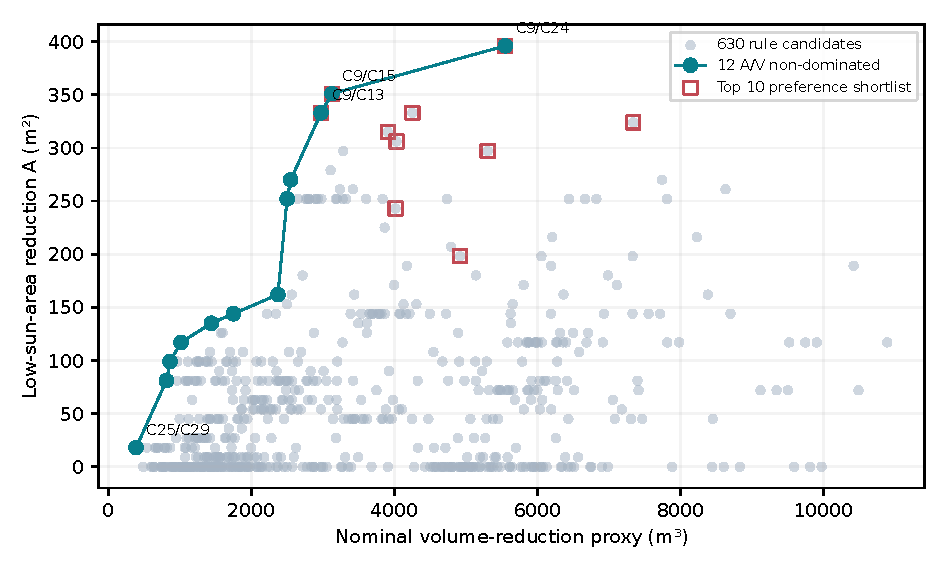
\includegraphics[width=\textwidth]{figures/candidate_tradeoff.pdf}
\Description{Full candidate universe plotted by nominal volume proxy and low-sun-area reduction, with the top ten and nondominated candidates highlighted. The plot displays the finite modeled choice set, not site geometry.}
\caption{The complete area--nominal-volume choice set, recomputed from archived candidate aggregates. The top ten follow the four-term score; the Pareto front uses only $A$ and $V$. This aggregate plot contains no site coordinates or newly simulated observations.}
\label{fig:choice}
\end{figure}

All twelve nondominated candidates have nonzero area benefit. Three also appear in the top ten, giving nineteen distinct score-selected or Pareto candidates. Adding historical pairs C6/C33 and C13/C24 and reference pairs C3/C19 and C26/C35 yields the curated 23. The reference pairs are interventions used for comparison; they are not the unchanged baseline scene. This review pool covers 23/630, or approximately 3.65\%, of the rule universe. The fraction describes selection effort, not verified global recall or a measured saving in the whole design process.

Every top-ten rule has an archived Honeybee result. Area reduction agrees exactly for nine of the ten; C9/C27 has $324$~m$^2$ in screening and $333$~m$^2$ in the archived rule review. Design-translation evidence is much narrower: only C9/C24 and C9/C15 have checked contained corrections, while C9/C13 reuses an already-contained result. The other seven rows have no archived translated-design verification. In particular, the first-ranked rule's $396$~m$^2$ result must not be mistaken for the corrected translation's $351$~m$^2$. A reviewed rule is evidence for further assessment, not a completed design.


\subsection{Agreement within Preserved Cohorts}
Table~\ref{tab:agreement} separates the two cohorts and the three compared metrics. For low-sun-area reduction, the curated cohort has Spearman $\rho=0.999258$ and the coverage cohort $\rho=0.997668$. In the latter, 19 candidates agree exactly and one differs by 9~m$^2$, yielding MAE 0.45~m$^2$. This is an average candidate-aggregate error on a grid with 9~m$^2$ cell weights; it is not sub-grid spatial precision.

\begin{table}[tbp]
\caption{Descriptive same-metric agreement with archived Honeybee aggregates. Statistics are recomputed from frozen tables; no new cohort simulations are implied.}
\label{tab:agreement}\centering
\begin{tabular}{llrrr}\toprule
Cohort & Metric & Spearman $\rho$ & MAE & Exact matches\\\midrule
Curated ($n=23$) & $A$ (m$^2$) & 0.999258 & 0.391304 & 22/23\\
 & $H$ (h) & 0.991597 & 0.001177 & 3/23\\
 & $S$ & 0.999012 & 0.006933 & 3/23\\
Coverage ($n=20$) & $A$ (m$^2$) & 0.997668 & 0.450000 & 19/20\\
 & $H$ (h) & 0.999624 & 0.000295 & 9/20\\
 & $S$ & 1.000000 & 0.002139 & 9/20\\\bottomrule
\end{tabular}
\end{table}


Coverage-cohort score ranks agree perfectly, but the score values do not: MAE is 0.002139 and only 9 of 20 scores agree exactly. Moreover, $V$ is shared between routes and $N$ is constant. The score comparison cannot validate four independent performance criteria, and correlation one cannot be read as 100\% predictive accuracy. The exposure routes also have different effective solar vectors. Their high aggregate agreement is useful evidence for this frozen screening task, with those qualifications.

Tie handling materially affects the top-five $A$ comparison within the 20-candidate coverage cohort. Here overlap is divided by five for exact-five sets. The retained legacy source-order result of 0.8 becomes 1.0 under the specified natural-pair exact-five rule, while including all boundary ties produces sets of six and seven candidates. This is a change in set definition, not an improvement in the physical model. We consequently avoid presenting a single top-five overlap as a universal selection guarantee. Likewise, an older correlation that compared score ranks to area ranks is not compared to the present same-metric correlations as evidence of progress.

\subsection{Measured Reuse Efficiency}
All 12 measured scale/repeat comparisons pass pointwise and aggregate equivalence checks. Table~\ref{tab:runtime} reports the scale-level medians. At 630 candidates, repeated intersection takes 11,608.183~s and reuse takes 24.037~s including precomputation; their ratio is 482.927. The relative benefit increases with the candidate count as repeated geometry work accumulates while preparation is amortized.

\begin{table}[tbp]
\caption{Measured end-to-end runtime medians from three single-thread repeats at each size. B includes precomputation. Ratios compare these implementations only.}
\label{tab:runtime}\centering
\begin{tabular}{rrrrr}\toprule
Candidates & Repeats & A (s) & B (s) & A/B\\\midrule
5 & 3 & 109.706 & 23.359 & 4.697\\
20 & 3 & 373.812 & 23.418 & 15.963\\
60 & 3 & 1,085.983 & 23.975 & 45.297\\
630 & 3 & 11,608.183 & 24.037 & 482.927\\\bottomrule
\end{tabular}
\end{table}


This is an implementation comparison, not a general solver comparison. In particular, the repeated-intersection implementation is not a spatial-index baseline, and the experiment does not time equivalent Honeybee scenes against B. Historical screening and Honeybee timings with different machines, solver semantics or worker counts are excluded from the ratio. The result supports the benefit of reuse in the measured setting, while leaving the benefit relative to other optimized implementations unmeasured.

The current archive reanalysis preserves the historical candidate ordering, all ten shortlist identities and the twelve-member Pareto front. The six saved full-universe A/B aggregate files are byte-identical. Recomputed scores agree with saved scores to floating-point rounding, with a maximum absolute discrepancy below $10^{-14}$. These are consistency checks on archived numbers, not a new execution of geometric intersections or evidence of fidelity to the physical site.

\subsection{Translation Failure and Controlled Correction}
Four of five historical translations fail the solid-containment check. In C9/C24 and C13/C24, rays that were clear in the baseline intersect upper walls of C24 outside its original footprint. Each of these scenes has four worsened receiving points and 9~m$^2$ of newly low-sun grid area in the retained historical result. The actual ray hits identify added obstructions as the cause. Synthetic tests had also exposed hole-handling and silent-face risks, but the canonical site has no holes and the six archived face dictionaries regenerate exactly; those synthetic defects are not asserted as the cause of this case.

The four contained corrections have no adverse visibility events, worsened receiving points or newly low-sun grid area on the fixed model, rays and grid. Figure~\ref{fig:translation} retains the before/after distinction. Low-sun-area reduction changes from 342 to 351~m$^2$ for C9/C24 and from 207 to 216~m$^2$ for C13/C24. C9/C15 and C6/C33 remain at 342 and 18~m$^2$. The already-contained C9/C13 remains at 333~m$^2$ through reuse of its unchanged historical result, not an additional correction run.

\begin{figure}[tbp]\centering
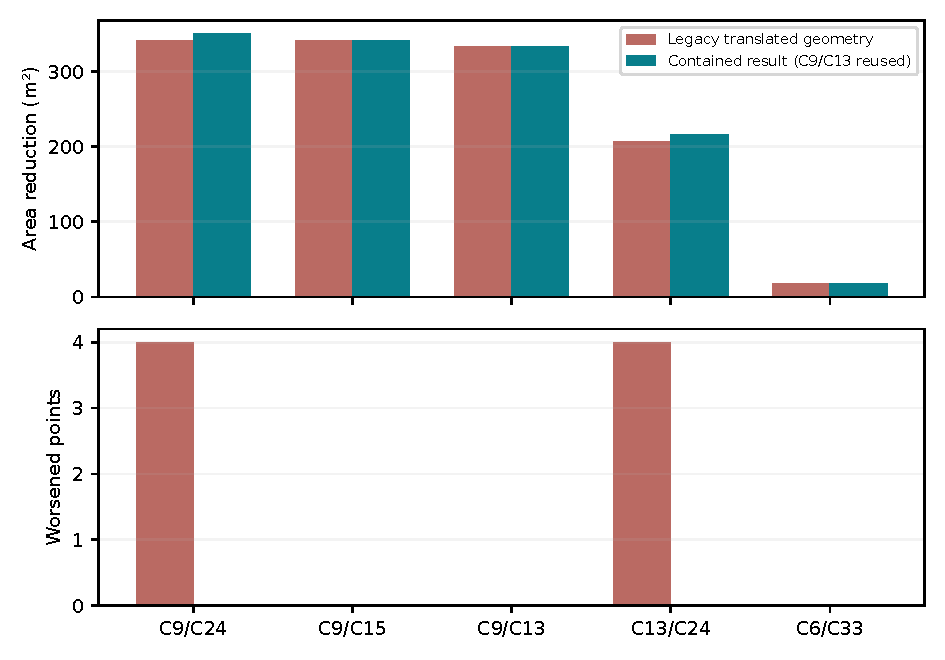
\includegraphics[width=\textwidth]{figures/translation_publication.pdf}
\Description{Five paired historical and corrected displays. C9/C24 and C13/C24 improve area reduction by nine square metres and reduce worsened points from four to zero. The C9/C13 corrected display reuses an unchanged historical result.}
\caption{Controlled translation recheck. Top: low-sun-area reduction relative to baseline. Bottom: worsened receiving-point count. Four corrections were simulated in the historical recheck; C9/C13 is already contained and reuses its unchanged result. The historical adverse results remain visible; the comparisons are not volume matched.}
\label{fig:translation}
\end{figure}

For any translated solid, the signed net union-volume reduction is $|\Omega_0|-|\Omega_c|$. For a noncontained legacy solid, this equals removed baseline volume minus added outside volume; it is not gross removed material. Table~\ref{tab:volumes} shows why containment correction must not be called a volume-matched comparison. Nominal rule budgets, rule-solid net union-volume reduction and translated-solid net union-volume reduction differ. C6/C33 is particularly informative: its nominal additive proxy is 5,583.055~m$^3$, while uniform-rule net union-volume reduction is 1,909.864~m$^3$ and corrected translation net union-volume reduction is 2,554.767~m$^3$. These quantities characterize the frozen approximate solids, not verified demolition or construction quantities. Similar area outcomes do not imply geometrically equivalent interventions.

\begin{table}[tbp]
\caption{Volume distinctions in the canonical model (m$^3$). The nominal column is additive per building; other columns use signed whole-scene net union-volume reductions. C9/C13's correction column reuses its already-contained result.}
\label{tab:volumes}\centering
\begin{tabular}{lrrrr}\toprule
Pair & Nominal rule & Rule union & Legacy union & Corrected union\\\midrule
C9/C24 & 5,551.333 & 5,470.406 & 5,259.615 & 5,474.582\\
C9/C15 & 3,127.755 & 3,065.681 & 2,927.693 & 2,937.931\\
C9/C13 & 2,975.156 & 2,918.246 & 2,785.422 & 2,785.422\\
C13/C24 & 3,863.880 & 3,726.044 & 3,534.257 & 3,749.224\\
C6/C33 & 5,583.055 & 1,909.864 & 2,553.509 & 2,554.767\\\bottomrule
\end{tabular}
\end{table}

\FloatBarrier
\section{Discussion and Limitations}
\subsection{Using the Shortlist in Architectural Work}
The immediate value of the workflow is a smaller, documented choice set.\aidraft{} An architect can compare candidate identities and benefits without manually creating 630 detailed models, while retaining the option to inspect the whole universe. The score provides one declared ordering; the Pareto set keeps lower-volume alternatives visible. The review status identifies which numbers have a second computational route and which translated forms still require assessment. This is a proposed use of the outputs, not a measured reduction in architects' working time or evidence from a user study.

The next practical decision is not necessarily to select rank one. The architect may reject a highly ranked pair because the modeled eligibility flag does not reflect ownership, function, protected fabric or structural constraints. A lower-ranked candidate may merit further work for reasons not represented in $A/H/V/N$. Those judgments should be recorded alongside, rather than hidden inside, an unexplained change to the score. If the team changes the modeled eligibility, geometry, rule, threshold or preference scenario, the result becomes a new explicitly versioned analysis; the frozen results should remain available for comparison.

Translation is a further decision gate. The historical C9/C24 result illustrates why adverse sunlight cannot be accepted uncritically as the natural price of a subtractive intervention. Actual rays hit walls that had been generated outside the baseline footprint. Containment and re-evaluation corrected that error, while volume accounting showed that clipping was not volume matching. Consequently, the updated evidence does not justify a permanent rule that only previously favored pairs may proceed. It supplies corrected outcomes for comparison and requires the architect to examine the intended intervention, verified boundaries and relevant costs.

Fast evaluation makes this bounded review process computationally practical under the measured conditions, but it does not solve omitted decisions. The 24.037~s historical implementation time concerns the canonical 630-rule calculation and includes blocker preparation. It excludes an architect's model preparation, stakeholder consultation, structural investigation and detailed design. The broader human workflow was not timed. The contribution is therefore an auditable computational component for early selection, with explicit handoff information and limits.

\subsection{Threats to Validity}
\paragraph{Canonical geometry.} The DXF component-bounding-box unions, shared components, overlapping footprints and OBJ disagreements are the most important external-validity limits. Reproducing a canonical model across implementations cannot validate its as-built fidelity. Correcting those boundaries would define a new input version and require an explicit assessment of affected results. Current cohort agreement must not be transferred to that new geometry without evidence.

\paragraph{Restricted physical scope.} A single day, 16 samples, a 3~m grid, a 0.1~m receiving height and an assumed north orientation delimit the reported performance. Threshold counts can change discontinuously near 3~h. The constant WEA carrier is not measured meteorology, and the study does not validate indoor illuminance, glare, annual weather, energy production or regulatory compliance. The distinction between saved pvlib rays and archived Ladybug rays remains part of the cross-route comparison rather than being suppressed to imply identical astronomical inputs.

\paragraph{Comparison design.} The matched timing comparison controls the geometric primitive and single-thread execution, but covers only one canonical model and two implementations without spatial indexing. Three repeats quantify the recorded execution conditions; they do not characterize hardware populations or arbitrary polygon complexity. We do not claim a measured memory reduction from the analytic blocker-array size or unavailable RSS values. A stronger efficiency comparison would include indexed and compiled baselines with the same accounting contract.

\paragraph{Cohorts and metrics.} Curated review and outcome-blind coverage serve different purposes and remain separate. Neither is a random multi-site sample. Shared volume inputs, constant $N$, discretized area, ties and preference weights constrain the interpretation of rank agreement. Candidate-level aggregate errors can mask spatial differences. The frozen 20 were not selectively rerun after the translation audit because no shared receiver, temporal-parser or missing-face defect was found in the actual scenes. A newly demonstrated shared defect would require an affected-scope review rather than selective retention of favorable outputs.

\paragraph{Correction scope.} Four corrected translations remove the observed adverse events under fixed rays and receivers. This supports the tested containment correction on this canonical model, not a guarantee for arbitrary imported meshes. Containment does not ensure equal volume, structural feasibility or a preferred design. The nominal $V$ proxy should be replaced or supplemented by an appropriate audited quantity if the decision requires physical removal costs.

\subsection{Reproducibility and Responsible Release}
The evidence separates historically measured runtime and scene replays, current frozen-table recomputation and reused historical results. Run identifiers, source, configuration and input hashes, raw timing repeats, aggregate tables, equivalence checks, correction ledgers and figure-source manifests are retained. The final integrated test record contains 112 passing tests; this supports software regression coverage, not physical ground truth. Failures and amendments remain part of the record rather than being overwritten.

Raw CAD, DXF, SKP and OBJ inputs, receiver coordinates, WEA carriers, Honeybee models and Radiance intermediate data remain restricted. Figures in this manuscript show aggregate evidence without site geometry or receiver coordinates. No public artifact release or unrestricted replication right is asserted. Any external evidence package must be reviewed for rights and anonymity before distribution. This restriction limits independent reproduction of the site-specific experiment and should remain visible alongside the available aggregate and algorithmic detail.

\section{Conclusion}
This study returns a bounded solar-access search to the architectural decision it supports: which interventions deserve further examination?\aidraft{} Under fixed research eligibility and height rules, all 630 building-pair candidates are evaluated, a score-based top ten and area--volume alternatives are exposed, and a curated 23-candidate review pool links screening to archived Honeybee/Radiance evidence. The resulting choice set preserves the distinction between a ranked rule, a reviewed rule, a checked translation and a professionally acceptable intervention.

Historical supporting experiments make that workflow more auditable. Two matched implementations preserve pointwise and aggregate results while reducing the full-universe median runtime from 11,608.183 to 24.037~s, including reuse preparation. Preserved same-site cohorts show strong aggregate agreement within their sampling and metric limits. Controlled translation replays identify erroneous outside-footprint obstructions, and four contained corrections remove the observed adverse events on the fixed rays and grid. The current cloud reanalysis reorganizes and recomputes archived evidence; it adds no new site simulation.

The workflow does not establish as-built accuracy, statutory compliance, volume-matched construction quantities or an automatically approved design. Its next substantive extensions are verified boundaries, broader site and preference coverage, additional optimized computational baselines and direct evaluation of how architects use the shortlist. For the present case, its defensible output is a transparent range of candidates and review evidence that an architect can scrutinize before deciding what to develop.

\section*{Acknowledgments: AI-Assistance Disclosure}
An OpenAI assistant~\cite{openai2026} provided substantial assistance with the abstract and Sections~1--8, including evidence organization, narrative restructuring, text generation and editing, mathematical presentation, table preparation, figure descriptions, bibliography checks, and analysis and LaTeX quality-control code. Section-specific citations identify this assistance. Numerical tables derive from archived measurements and explicit aggregate recomputation; no observations were invented to complete missing experiments. Diagram and chart preparation uses workflow descriptions and recorded aggregates rather than generated site imagery. The exact underlying model version was not recorded. This statement describes preparation of this draft and does not assert that the authors have completed independent verification or approved its content. Author review and responsibility remain required before submission.

\FloatBarrier
\bibliographystyle{splncs04}
\bibliography{references}
\end{document}
